\subsection{Attēlu raksturpunktu salāgošanas algoritmi} \label{sec:matching}
\begin{figure}[tbh]
	\centering
	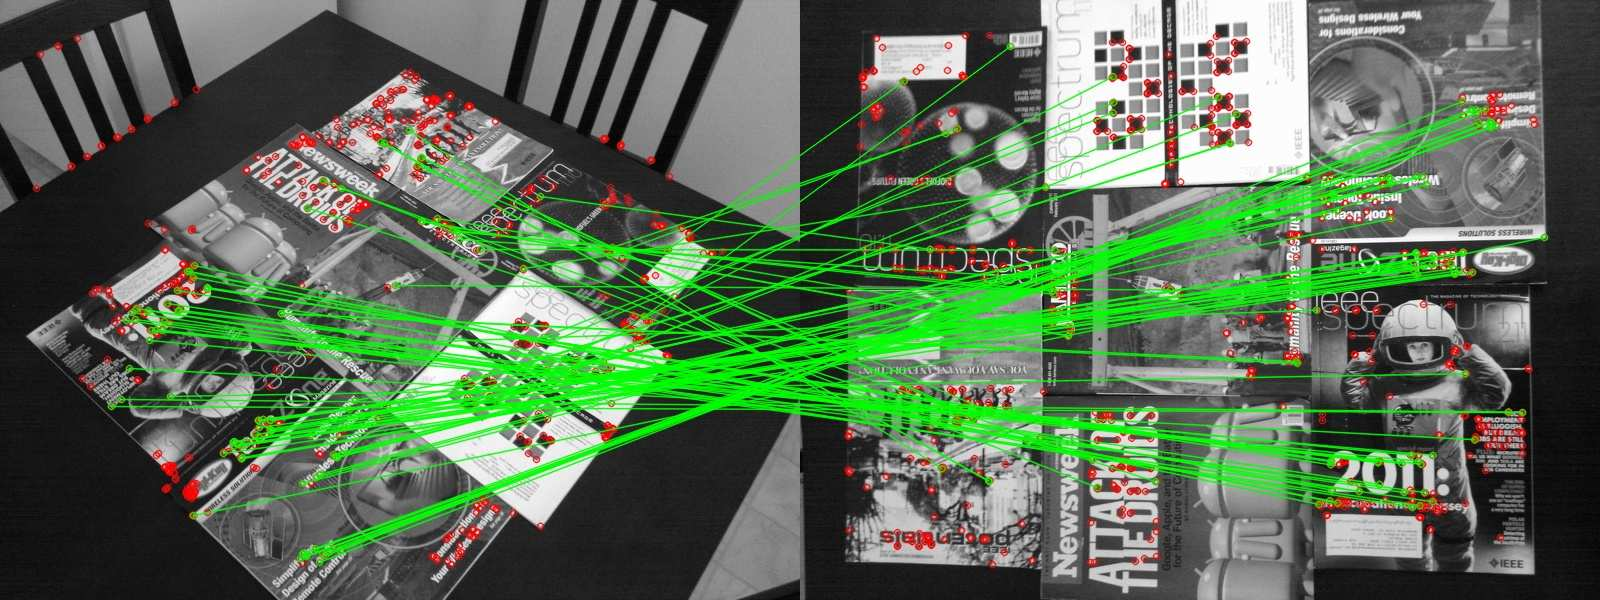
\includegraphics[width=0.8\textwidth]{orb-match}
	\caption{Attēlu pāra raksturpunktu salāgošana ar ORB~\cite{ORB}.}
	\label{fig:orb}
\end{figure}

Raksturpunktu salāgošana ir punktu pāru (vai kopu) atrašana divos
(vai vairākos) attēlos, kuri atbilst vienam un tam pašam attēlā redzamam
objektam. Salāgošanas piemērs redzams \ref{fig:orb}~attēlā, kur ar zaļu
savienoti salāgotie raksturpunktu pāri un ar sarkanu apzīmēti raksturpunkti,
kuriem pāris nav atrasts.

Raksturpunktu salāgošana tiek izmantota tādos mašīnredzes pielietojumos, kā
% TODO: citēt pielietojumus
objektu atpazīšanā un sekošanā, attēlu ,,sašūšanā'', 
telpiskās informācijas rekonstrukcijā (kartēšanā) no attēliem,
vienlaicīgā pašlokalizācijā un kartēšanā (SLAM), u.c..

Raksturpunktu salāgošanas pamatā ir šo punktu ,,aprakstīšana'' izveidojot
raksturpunkta \termTech{deskriptoru}, kas satur informāciju,
kas ir pietiekami unikāla, lai nesakristu ar citiem raksturpunktiem attēlā
un ir noturīga pret sagaidāmām attēla īpašību izmaiņām.
\termEn{Deskriptoram} tātad nepieciešamas vai vēlamas šādas īpašības:
\begin{itemize}
	\item \newTerm{\emph{diskriminitāte}} --- spēja izšķirt raksturpunktus
		pēc to \termTech{deskriptoriem};
	\item \emph{pozīcijas invariance} --- spēja salāgot raksturpunktus
		neatkarīgi no tā koordinātēm attēlā;
	\item \emph{rotācijas invariance} --- spēja salāgot raksturpunktus
		neatkarīgi no attēla rotācijas leņķa;
	\item \emph{intensitātes invariance} --- spēja salāgot raksturpunktus
		neatkarīgi no globālas intensitātes izmaiņas;
	\item \emph{mēroga invariance} --- spēja salāgot raksturpunktus
		neatkarīgi no mēroga (attēla izmēru un/vai raksturpunkta objekta attāluma izmaiņa);
	\item \emph{perspektīvas invariance} --- spēja salāgot raksturpunktus
		neatkarīgi no perspektīvas (attēla uzņemšanas pozīcijas izmaiņa);
	\item \emph{trokšņu noturība} --- spēja salāgot raksturpunktus
		attēlā (iespējami) neatkarīgi no ,,trokšņa'' līmeņa attēlā;
\end{itemize}
Ir norādītas vairākas attēla izmaiņu invariances īpašības,
kas nozīmē ka tās nevar izmantot lai aprakstītu raksturpunktu.
Variance ir nepieciešama lai nodrošināti diskriminitāti un, praktiski visos
algoritmos, tiek izmantota lokālas intensitātes izmaiņas attēlā 
rakturpunkta tuvējā apkārtnē.

Eksistē vairāki algoritmi \termTech{deskriptoru} izgūšanai un
salīdzināšanai, t.sk.,~%
SIFT, % FIXME: Vai SIFT arī apzīmē deskriptoru?
SURF, BRIEF un tā varianti, ORB, u.c..
Algoritmus var izvērtēt pēc jau uzdotajām īpašībām, 
bet jāņem vērā arī to veiktspējas īpašības:
\begin{itemize}
	\item \emph{skaitļošanas kompleksitāte}, kas tieši ietekmē laiku
		kurā viens attēls var tikt apstrādāts;
	\item \emph{informācijas blīvums}, kas atspoguļo cik liela ir katra
		informācijas bita variance, kas ļauj sasniegt lielāku diskriminitāti
		pie mazāka bitu skaita.
\end{itemize}

Šajā darbā, ORB ir izvēlēts par algoritmu, kura veiktspēju salīdzināt uz
dažādām aparatūras platformām. ORB izvēlēts, jo tā raksturpunktu salāgošanas
spēja ir līdzīga vai labāka nekā SIFT, bet ir par divām kārtām ātrāks nekā
SIFT un par kārtu ātrāks nekā SURF \cite{ORB}.
ORB izmantotais rBRIEF \termTech{deskriptors} ir
noturīgāks pret troksni nekā SIFT un tā rotācijas invariance līdzvērtīga SIFT.


